\documentclass{csfourzero}

\title{Impact of Meltdown \& Spectre Mitigations}
\author{Konrad Dryja}
\date{\today}
% A useful package to support on-line references
\usepackage{url}
\usepackage{natbib}
\usepackage{xcolor}
\usepackage{listings}
\usepackage{enumitem}
\usepackage{booktabs}
\usepackage{subfigure}
\lstset{language=C,keywordstyle={\bfseries \color{blue}}}
\bibliographystyle{plain}
\abstract{In my CS4040 report I'd like to evaluate the impact of the discovery of Side-Channel Attacks back in January 2018 with Spectre \& Meltdown leading. As those were utilizing many of the performance reliant features - which had to be rolled back or squashed due to security concerns. The removal resulted in many reports about grossly deteriorated performance. With the patches already in place, I have gone ahead and removed them to compare before and after performance of one- and multi-core performance in different tasks, such as prime calculation or rendering. I will be aiming to diversify tested hardware and software, including platforms such as Windows, Linux and Intel, AMD. Final points will close off the results, concluding with recommendation whether it's reasonable to leave the mitigation disabled in lights of potential vulnerabilities.}


\begin{document}
\maketitle


\section{Introduction}
\label{sec:intro}
Speculative execution is a feature that was included in modern CPUs by almost all chip designers, significantly boosting the execution time on some very complex operations. With time, those solutions became more and more aggressive, as the competition between manufacturers was very fierce, fighting to beat the competitors in benchmarks, thus winning the favours of reviewers \& consumers.

Perhaps one of the most daunting days that security professionals faced happened on January 3rd, 2018 - when Meltdown \& Spectre attacks were publicized, explaining a serious flaw with speculative execution approach. With the enhancement no longer considered safe, modern CPU manufacturers were forced to drop these features in favour of enhancing security. But at the same time, it resulted in sacrificing the performance of the chips. Probably the most harming aspect was that speculative execution was at the time an industry standard. 

Personally, I found the topic the most interesting, as the aftermath is still haunting security researches to this day, since the fault was not the software, but inherent architecture was found to be flawed. Moreover, nowadays we are frequently hearing news (most recent being "Fallout"\cite{fallout}) how the newest vulnerability based on side-channel execution has been discovered - with the definite fix being complete hardware replacement with a chip produced after 2017. This forced Intel, AMD, ARM to release very aggressive patches, greatly hurting the benchmarks.

This has also raised ethical questions - since some of the affected machines suffered as much as 50\% drop in performance. In the eyes of law, this could classify as false advertising which naturally was followed by many class-action lawsuits. As stated by Intel in their 2017 Annual report, as of February 2018, they were facing 30 customer suits along with two securities \cite{intelreport}. Intel perhaps is the company that was the most under fire, since Variant 1, also known as Meltdown, was mostly apparent in their chips, although Variant 2 \& 2 were replicated in almost all consumer chips (including AMD et al.).

Computing community and hardware architects were faced with a difficult dilemma - how much of security are we willing to sacrifice in favour of increased performance?

\section{Background and related work}
\label{sec:lit}

When speaking about Spectre and Meltdown, it's very important to start from the very beginning - when in July 2017, a researcher Jann Horn from Google's Project Zero has discovered the vulnerability. Due to the severity and potential implications resulting from premature releasing of the findings, those were first communicated directly - on NDA basis - with manufacturers, hoping for an immediate fix. On January 2018, two papers were released by J. Horn et al. illustrating in-depth the vulnerabilities and how they could be replicated \cite{Lipp2018meltdown, Kocher2018spectre}. The papers present a throughout overview of the potential attack - the exploitation here is based on \textbf{Branch Prediction} (BP) along with \textbf{Out of Order Execution} (OOE). Those are optimizations techniques used by almost all CPUs on the market:

\begin{itemize}[noitemsep]
  \item BP lets the processor "predict" direction where the program's execution flow will go towards without explicitly evaluating the condition. For example, in a situation where \lstinline{if} statement was successful for 100 iterations, it can assume that 101st will be successful as well and thus prematurely execute the included code-block, storing the result in L-cache (high speed, low capacity memory located directly on the CPU core)  
  \item OOE, on the other hand will often reorder scheduled operations leaving the most time-consuming actions till the end, executing the ones containing required data present in CPU cache immediately - assuming that those do not depend on each other, e.g., it's a simple summation, not relying on the prior information.
\end{itemize}

Together, they create a cheap and clever way to speed up the execution of binaries, but unbeknownst opened a pathway for side-channel attacks, exploiting the fact that CPU was executing the code that it wasn't meant to in the first place. Normally, the results are only stored in fast-access L-cache (which is only accessible from kernel-mode and is purely used to increase performance), with no way to read those blocks from user mode. A proof-of-concept presented by the researches \cite{Kocher2018spectre} illustrated how it's possible to measure how long it takes to access particular variable in order to determine whether it's coming from RAM or L-cache and then make statistical assumption whether the piece of data was evaluated inside of block of code which was executed speculatively. 

There is also a subtle difference between the nature of attacks described by \textbf{Meltdown} (Variant 3) and \textbf{Spectre} (Variant 1, 2). The former allowed for any arbirtary process to access kernel-space memory, which contains restricted data such as password or even latest keystroke information. The latter - on the other hand - was capable of crossing process or sandbox boundaries, effectively nullyfying the protections provided by virtualised environment or JIT (just-in-time) compilers. This potentially might allow an attacker to deploy malicious binary onto VM cluster (run by a cloud provider such as GCP or AWS) and access information of other users.

\begin{lstlisting}[caption=Meltdown PoC,frame=tlrb, numbers=left, firstnumber=1]{Name}
char testArray[256 * 64];
evictCache(testArray); // Clear L-cache
char x = * kernelSpace; // Will cause segmentation fault
testArray[x * 64]++; // Will be executed speculatively
for(int i=0; i<256; i++) {
  // Measure how long it takes to access the element
  if(is_cached(testArray[i * 64]) {
    // Cache hit! Found secret bit.
  }
}
\end{lstlisting}

Multiple patches have been created ever since to mitigate the negative effect, trying to minimize the impact on performance. M. L{\"o}w\cite{low2018overview} provides an overview of created mitigations and affected hardware. The major and immediate patches which had the biggest performance effect included:

\paragraph{KAISER} \cite{corbet2017current} - which stands for Kernel Page-Table Isolation. Meltdown is exploiting the fact that for the purposes of reduced access times, the entire kernel address page is mapped to every process. This is not directly accessible from user-mode and is protected by privileged bit. Unfortunately, with side-channel attacks, this data can be speculatively loaded and then later retrieved via a covert channel. KAISER aims to drop that mapping and leave only necessary signals.
\paragraph{Retpoline} \cite{turner2018retpoline} - retroactive trampoline, it's a mitigation aiming to catch Branch Predictor in an infinite loop, effectively never speculatively executing sensitive code.

It is also important to mention that software mitigation can only be helpful to a specific point. From month to month more ways of performing side-channel attacks are discovered, bypassing completely the mitigations, thus manufacturers are force to deploy more and more restrictive patches, decreasing the benefits of BP and OOE.


\section{Research question}
\label{sec:rq}
Having introduced the basics of side-channel attacks in previous sections, we are now ready to tackle the implications of the released patches. The research question that could be formed following the aforementioned considerations would be \textbf{`` How significant the performance degradation was, after mitigations for Side-Channel Attacks had been deployed? ``}. 

Fortunately, majority of the flaws were already patched with immediate effect, meaning that the vulnerability cannot be replicated on up-to-date software. This leaves us with necessity of either simulating the hardware via software or rolling back the updates. To this day, Dell claims that no malicious use has been spotted to this day \cite{dell}, which introduces question of how severe the incident was and whether the sacrifice was worth it. We can speculate that this announcement and others pushed the Linux team to introduce an option for kernel versions starting from 5.2 allowing the users to disable the mitigations, regaining the performance but opening the system for potential attacks.  

\begin{lstlisting}[caption=Vulnerable Linux system with disabled mitigations,frame=tlrb,language=bash]{Name}
% lscpu            
[...]
Model name:                      Intel(R) Core(TM) i5-6500 CPU 
[...]
Vulnerability L1tf:              Mitigation; PTE Inversion;
Vulnerability Mds:               Vulnerable; SMT disabled
Vulnerability Meltdown:          Vulnerable
Vulnerability Spec store bypass: Vulnerable
Vulnerability Spectre v1:        Vulnerable:
Vulnerability Spectre v2:        Vulnerable, IBPB: disabled
\end{lstlisting}

For Windows, on the other hand, the mitigations are slightly harder to disable, although it can be achieved by tweaking Windows Registry \cite{msoft}. While the impact on consumer Windows version can be negligible (according to Microsoft\cite{myerson2018understanding}), Server edition of their Operating System was particularly susceptible to slowdowns, especially during Input/Output operations. Microsoft decided to leave the decision of enabling the patch up to system administrators, leaving the option enabled by default. Alas, mitigations for CVE-2017-5753 (Spectre Variant 1) cannot be disabled for Windows at the moment. To work around this, it is still possible to install Windows 10 Version 1607 (From April 2016) and perform all experiments in that environment - with no internet connection to avoid automatic updates. Although this might also cause inconsistency, as newer revision might also have included unrelated performance fixes - thus the test would have to be performed on both older revision of Windows 10 and Windows Server with only disabled mitigations.

At this point, with a vulnerable system, we have several ways to obtain before-after comparison of performance, as mentioned: each platform offering different solutions. Linux has open access to compiled byte-code with an option of disabling optimizers potentially spoiling the results. Usually, to benchmark the performance of a CPU, we would be looking at how quickly it can solve complex operations. One of the examples being prime numbers calculations or matrices multiplication. There are two open-source packages which wrap around those operations, producing a concise report on performed CPU Cycles, page faults, thermal readings etc. - stress-ng \cite{stressng} and sysbench \cite{sysbench}  

With Windows, it is slightly more difficult to access direct CPU registers from the OS - additionally, all the compiled code is subject to many optimizations, which might introduce variance and inconsistencies in the results. The most efficient way would be to utilize closed-source, proprietary software created specifically for benchmarking (used mostly to compare and rank consumer-grade products), which can extract raw performance data. Most popular choice nowadays is Cinebench along with 3DMark which at the same time could determine whether the slowdowns in CPU could also be affecting external GPU.

For the purposes of this research, I will be focusing only on readings obtained from hardware running Linux operating systems, in order to prevent potential noise created by possible performance gains patched alongside Spectre mitigations.

\section{Experimental Design}
\label{sec:exp}
In order to answer the research question and evaluate how big and whether meaningful the impact was, we can devise the following null hypotheses: 
\begin{itemize}
  \item For each of the benchmarking utilities run on the hardware, Spectre mitigations do not cause statistically significant differences in the results.
  \item Runtime of CPU-intensive operations (such as encryption) does not increase with enabled mitigations for Spectre.
\end{itemize}

Since the mitigations for the vulnerabilities described in previous sections heavily modify or straight-up disable a lot of performance features present in modern chips, it will be necessary to perform benchmarking on the CPUs themselves with and without those mitigations installed. Running generic speed tests on the performance of the chips side-to-side with the same CPU without the patches will result in potential runtime differences.

As I have access to two separate machines running Linux, I will be conducting all tests and benchmarks on them. Since their CPUs and specifications vary, it is important to note it down as an independent variable in the experiment - as the results will vary on both machines. Although, what we are interested in, is the difference before and after applying the patch, rather than raw comparison between those two machines; for example, Machine A will be outperforming Machine B - but we are not interested in that.


\begin{table}[h]
\centering
\begin{tabular}{|l|l|l|ll}
\cline{1-3}
    & Machine A (Workstation)         & Machine B (Laptop) &  &  \\ \cline{1-3}
CPU & i5-6500 @ 3.20GHz & i7-8550U @ 4.00GHz       &  &  \\ \cline{1-3}
RAM & 16GB DDR4 2400MHz & 16GB DDR4 2400MHz          &  &  \\ \cline{1-3}
GPU & GeForce GTX 1070  & Intel UHD 620          &  &  \\ \cline{1-3}
\end{tabular}%
\caption{Specifications of testing population}
\label{tab:machines}
\end{table}

Table \ref{tab:machines} describes the exact specification of the hardware that I used for testing. Both are running 64-bit revision of Archlinux with the following versions: 

\begin{lstlisting}[frame=tlrb, basicstyle=\small]{Name}
% uname -a
Linux workstation 5.3.11-arch1-1 x86_64 GNU/Linux
% cat /etc/*release*
NAME="Arch Linux"
PRETTY_NAME="Arch Linux"
ID=arch
BUILD_ID=rolling
ANSI_COLOR="0;36"
HOME_URL="https://www.archlinux.org/"
DOCUMENTATION_URL="https://wiki.archlinux.org/"
SUPPORT_URL="https://bbs.archlinux.org/"
BUG_REPORT_URL="https://bugs.archlinux.org/"
LOGO=archlinux
\end{lstlisting}

Additionally, I had no access to hardware running other architectures, such as ARM or AMD, so those will also not be compared. Intel architecture was the one that was affected the most when it comes to Meltdown and thus the difference is going to be the most prominent on those chips.

Another important independent variable can be identified as benchmark / operation performed by the CPU. As there are various operations, sometimes abusing access to L-cache, or simply omitting it, I will be measuring performance with respect to different factors, such as context switching or ray tracing.

To maximise the significance of the results of my experiment, I will be looking to utilise the following testing suites, in addition to the ones that I have mentioned in the previous section:
\begin{itemize}
  \item \textbf{Phoronix Test Suite v9.2.0m2} - from within the suite, I will be running \textbf{Hackbench} (performance of communicating, scheduled tasks), \textbf{Stress-NG} (tests socket activity) and \textbf{ctx\_clock} (measures context switching) tests. Phoronix allows for multiple trial runs in order to establish p-value, I will be running each test 10 times.
  \item \textbf{Geekbench v5.0.4} - mostly geared towards simulating real-world scenarios, produces one and multi-core performance - tests are constructed with Augmented Reality and Machine Learning applications in mind. \cite{geekbench}
\end{itemize}
Each of them is capable of running and measuring expensive CPU operations such as Blowfish, Jack-The-Ripper password cracker or Text / Image Compression. As all of them incorporate various tests, they will produce different results. Depending on the benchmarking tool, either a numerical score is presented (Geekbench) or raw values in seconds to indicate the duration of given operation (Sysbench). All tests will be performed at least 10 times per machine, per patch installed / removed in order to establish statistical significance. 

Finally, to test the second hypothesis, it is possible to utilise the openssl binary found on almost every Linux system. Very handy sub-command called "speed" will continuously run various algorithms (MD5, SHA1, SHA256, SHA512, Whirpool) and measure how many hashes were successfully created in 3 seconds. In order to increase sample size, different sized blocks will be used (16, 64, 256, 1024, 8192, 16384)

To measure cryptographic efficiency for symmetric algorithms cryptsetup benchmark can be used. 

\begin{lstlisting}[caption=Versions of crypsetup and openssl, frame=tlrb, basicstyle=\small]{Name}
% cryptsetup --version
cryptsetup 2.2.2
% openssl version     
OpenSSL 1.1.1d  10 Sep 2019
\end{lstlisting}

The machines will be running under the same load with the same configuration installed. To eliminate potential noise, no unnecessary background programs will be running and if they are necessary, both before and after tests will have same runtime, which can be monitored using UNIX top command, also verifying load average. 

\section{Results}
\label{sec:results}

\subsection{Benchmarking suites evaluation}

\subsubsection{Phoronix Test Suite}

Starting off with \textbf{Hackbench} test, it was an experiment trying to stress the Linux kernel scheduler responsible for firing off and preparing new jobs for the CPU. Test was repeated for 10 times, for both Machines A \& B. Once compared the results from setup with enabled mitigations and the results from the one without, a $p-value$ can be obtained through Paired T-Test - $p_{a} = 6.25 * 10^{-14}$ and $p_{b} = 6.38 * 10^{-19}$, confirming statistical significance of my findings. 

\begin{figure}[h]
\centering
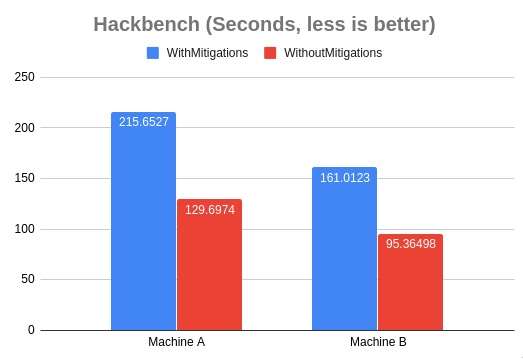
\includegraphics[width=10cm]{hack}
\caption{Results from Hackbench}
\label{fig:hackbench}
\end{figure}

Figure \ref{fig:hackbench} displays the exact differences between data when run with and without mitigations on both Machines. For Machine A we can observe almost 40\% regression after applying the patches and for Machine B the regression stands at 41\%. The results should be interpreted in ``less is better`` manner, as the numbers represent amount of time in seconds required to complete all scheduled tasks.


Moving on to the next part of Phoronix, which is \textbf{Stress-NG}. It used to be a part of the standard UNIX stress testing, used to verify whether the machine operates correctly over heavy load, albeit it can also be used to measure the number of operations per second it performs in a given timespan. Same as before, the test was repeated for 10 times, yielding the following $p-values$: $p_{a} = 3.13 * 10^{-30}$ and $p_{b} = 2.27 * 10^{-13}$ - in both cases, the value being less than $0.05$.

\begin{figure}[h]
\centering
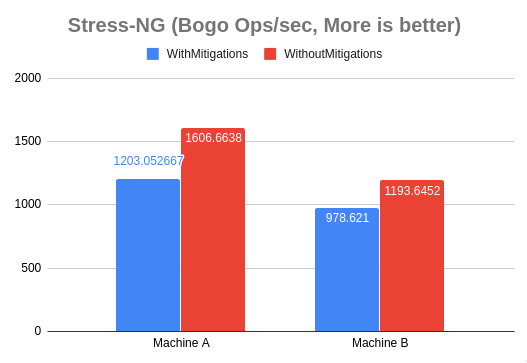
\includegraphics[width=10cm]{stress}
\caption{Results from Stress-NG}
\label{fig:stress}
\end{figure}

The regression is slightly less prominent in that situation, with Machine A performing approximately 25\% less of ``Bogus Operations``, along with Machine B performing approximately 18\% less. Contrary to the previous chart, higher number of performed operations indicates better performance, thus putting no mitigations systems at an advantage.   

Finally, \textbf{ctx\_clock} was also evaluated. In that particular case, number of clock cycles required for a context switch (e.g., from user mode into kernel mode) is measured. The test again has been repeated for 10 times, ending up with: $p_{a} = 1.08 * 10^{-21}$ and $p_{b} = 2.81 * 10^{-25}$, confirming significance.

\begin{figure}[h]
\centering
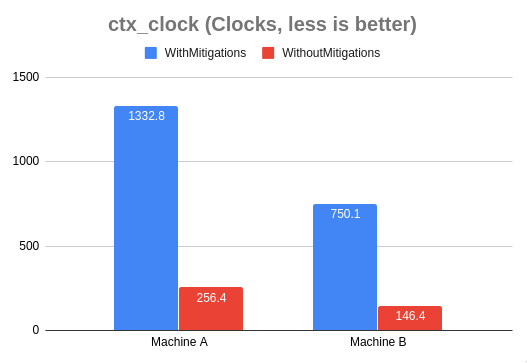
\includegraphics[width=10cm]{ctx}
\caption{Results from ctx\_clock}
\label{fig:ctx}
\end{figure}

For that case, the faster the context switch happens (i.e., requires fewer cycles), the better performing the chip is. Out of all three of the tests performed, the regression has been the most significant; with Machine A needing almost 420\% extra clock cycles and Machine B needing extra 80\%, when the patches for Spectre are enabled.

\subsubsection{Geekbench}

\textbf{Geekbench} is a fully equipped, all-in-one testing suite, often used for performance in Machine Leaning or gaming. As it's a commercially available benchmarking tool, additional tests are performed automatically and unfortunately $p-value$ of the results is not available - the only final outcome is the raw score of the machine. Moreover, the trial version that I was utilising permits only benchmarks on 32-bit applications, so the results may be different for 64-bit architectures.

\begin{table}[h]
\centering
\begin{tabular}{llr}
\cline{2-3}
\multicolumn{1}{c|}{}                   & \multicolumn{2}{c|}{Machine A}                                                 \\ \cline{2-3} 
\multicolumn{1}{l|}{}                   & \multicolumn{1}{l|}{WithMitigations} & \multicolumn{1}{r|}{WithoutMitigations} \\ \hline
\multicolumn{1}{|l|}{Single-Core Score} & \multicolumn{1}{l|}{1055}            & \multicolumn{1}{r|}{1052}               \\ \hline
\multicolumn{1}{|l|}{Multi-Core Score}  & \multicolumn{1}{l|}{3562}            & \multicolumn{1}{r|}{3547}               \\ \hline
                                        &                                      & \multicolumn{1}{l}{}                    \\ \cline{2-3} 
\multicolumn{1}{l|}{}                   & \multicolumn{2}{c|}{Machine B}                                                 \\ \cline{2-3} 
\multicolumn{1}{l|}{}                   & \multicolumn{1}{l|}{WithMitigations} & \multicolumn{1}{r|}{WithoutMitigations} \\ \hline
\multicolumn{1}{|l|}{Single-Core Score} & \multicolumn{1}{l|}{1064}            & \multicolumn{1}{r|}{1078}               \\ \hline
\multicolumn{1}{|l|}{Multi-Core Score}  & \multicolumn{1}{l|}{3892}            & \multicolumn{1}{r|}{3924}               \\ \hline
\end{tabular}
\caption{Scores reported by Geekbench}
\label{tab:geekbench}
\end{table}

Although, a T-Test can be performed against all different performed tests (21 * 2 in total) for Single and Multi-Core performance. If the tests were to be statistically significant, we would notice similar standard error and standard deviation between results. Sadly, it was not the case in this situation, with $p-values$ of $p_{a} = 0.0534765$ and $p_{b} = 0.072481043$ - in both situation the value being greater than 0.05 meaning that the obtained numbers yield no statistical significance.

I will be going into more depth as to what could've spoiled this particular test in the next section, but at first glance, we can predict negligible Spectre impact on operations needed for tasks such as AR / VR, which confirms the reports from earlier paragraphs mentioning that biggest impact would be on servers and their virtualisation capabilities, rather than end-user use cases.

\subsection{Cryptographic performance evaluation}

\subsubsection{OpenSSL}

OpenSSL was used to measure how many hashes the CPU is capable of creating in the span of 10 seconds. To establish statistical significance, for each hashing method the test was repeated for data blocks varying in size. After applying Paired T-Test to each of the 30 samples per Machine, following values were obtained: $p_{a} = 0.009730881344$ and $p_{b} = 0.02688339939$, in both cases $p < 0.05$, so the test holds statistical significance.

Figures \ref{fig:hashA} and \ref{fig:hashB} present the differences of standard deviations for each of the considered block size, when executed given hashing algorithm on Machine A or Machine B. The differences are minimal, with environments without mitigations performing slightly better, although the regression is less than 1\%. 

\begin{figure}[!h]
\centering
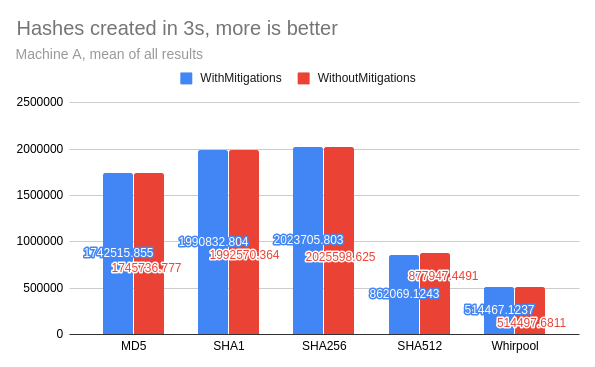
\includegraphics[width=15cm]{hashA}
\caption{Hashes created by Machine A}
\label{fig:hashA}
\end{figure}

\begin{figure}[!h]
\centering
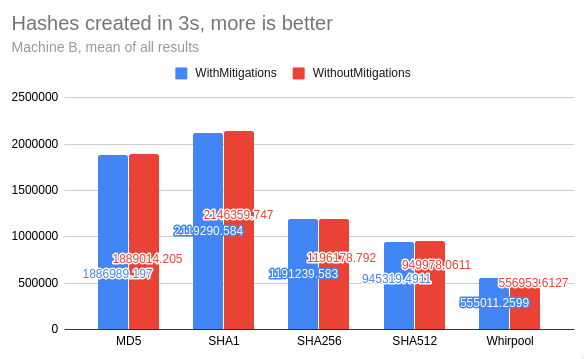
\includegraphics[width=15cm]{hashB}
\caption{Hashes created by Machine B}
\label{fig:hashB}
\end{figure}


\pagebreak

\subsubsection{Cryptsetup}

Contrary to OpenSSL, \textbf{cryptsetup} is capable of measuring the speed of modern, symmetric cryptographic algorithms. For the purposes for the experiment, most used and modern methods were used: AES-CBC, AES-XTS, Twofish-XTS and Serpent-CBC. Tables \ref{tab:cryptoA} \& \ref{tab:cryptoB} respectively present the mean results of all trial runs, on both test machines. Once performed paired T-Test, it was found that $p < 0.05$.

Carrying on, we notice the biggest impact on AES algorithms, with the most significant difference on AES-XTS using 512-blocks key, reaching even 957 MiB/s. On the other hand, Twofish and Serpent is more resilient to the mitigations, with differences of circa 15 MiB/s. 

\begin{table}[h]
\centering
\begin{tabular}{@{}lcrrrrr@{}}
\multicolumn{1}{c}{}          & \multicolumn{1}{l}{} & \multicolumn{2}{c}{WithMitigations}           & \multicolumn{1}{l}{} & \multicolumn{2}{c}{WithoutMitigations}                          \\ \cmidrule(r){1-4} \cmidrule(l){6-7} 
\multicolumn{1}{c}{Algorithm} & Key                  & Encryption   & \multicolumn{1}{l}{Decryption} & \multicolumn{1}{l}{} & \multicolumn{1}{l}{Encryption} & \multicolumn{1}{l}{Decryption} \\ \cmidrule(r){1-4} \cmidrule(l){6-7} 
AES-CBC                       & 128b                 & 1090.6 MiB/s & 3255.8 MiB/s                   &                      & 1123.2 MiB/s                   & 3443.5 MiB/s                   \\
AES-XTS                       & 512b                 & 1907.2 MiB/s & 1910.7 MiB/s                   &                      & 2761.5 MiB/s                   & 2759.7 MiBs                    \\
Twofish-XTS                   & 256b                 & 371.4 MiB/s  & 373.9 MiB/s                    &                      & 383.3 MiB/s                    & 385.4 MiB/s                    \\
Serpent-CBC                   & 256b                 & 93.9 MiBs    & 705.7 MiB/s                    &                      & 93.5 MiB/s                     & 712.3 MiB/s                    \\ \cmidrule(r){1-4} \cmidrule(l){6-7} 
\end{tabular}
\caption{cryptsetup benchmark on MachineA}
\label{tab:cryptoA}
\end{table}

\begin{table}[h]
\centering
\begin{tabular}{@{}lcrrrrr@{}}
\multicolumn{1}{c}{}          & \multicolumn{1}{l}{} & \multicolumn{2}{c}{WithMitigations}           & \multicolumn{1}{l}{} & \multicolumn{2}{c}{WithoutMitigations}                          \\ \cmidrule(r){1-4} \cmidrule(l){6-7} 
\multicolumn{1}{c}{Algorithm} & Key                  & Encryption   & \multicolumn{1}{r}{Decryption} & \multicolumn{1}{r}{} & \multicolumn{1}{l}{Encryption} & \multicolumn{1}{l}{Decryption} \\ \cmidrule(r){1-4} \cmidrule(l){6-7} 
AES-CBC                       & 128b                 & 1185.9 MiB/s & 3526.9 MiB/s                   &                      & 1203.9 MiB/s                   & 3749.7 MiB/s                   \\
AES-XTS                       & 512b                 & 2024.9 MiB/s & 2037.8 MiB/s                   &                      & 2981.7 MiB/s                   & 2988.8 MiBs                    \\
Twofish-XTS                   & 256b                 & 402.6 MiB/s  & 404.5 MiB/s                    &                      & 416.2 MiB/s                    & 417.8 MiB/s                    \\
Serpent-CBC                   & 256b                 & 101.1 MiBs   & 762.9 MiB/s                    &                      & 101.6 MiB/s                    & 780 MiB/s                      \\ \cmidrule(r){1-4} \cmidrule(l){6-7} 
\end{tabular}
\caption{cryptsetup benchmark on Machine B}
\label{tab:cryptoB}
\end{table}


\section{Discussion}
\label{sec:discuss}

Following the tests through Phoronix Suite, there is a clear regression visible for both Machine A and Machine B - the biggest being ctx-clock, which actually was excepted. We can suspect that KAISER (described in section 2) is at fault here - since the address space is no longer mapped directly to each process, the CPU has to compute all address spaces every time context switch is requested in order to switch from User to Kernel mode. For the remaining two tests, they were mostly benchmarking access times to virtual memory and how well the CPU is capable of handling page faults, again, task that was sped up by a magnitude thanks to speculative execution.

Interestingly, the Geekbench results had no significance, as the T-Test shown high probability of the differences being caused by random noise. This could have also been caused by the fact that I was using free version of Geekbench limited to only 32-bit instruction set along with limited control over repeated tests. It's an area definitely worth further exploration in order to determine the exact loss (or lack of it) on the tests performed by that software.  

Moreover, the cryptographic performance wasn't as impactful as the context switching or VM access times, with the exceptions of some algorithms (AES-XTS), the regression is less than 1\%. That's the operations most likely to be performed frequently by consumer-level hardware, with problems such as HTTPS/TLS connections being handled regularly.

We can observe see how swapping the variables - machine type and performed test - ends up with different results, yet with similar standard deviation. Moreover, in some situations Machine A was performing better and in others vice versa. This could hint towards the fact that 8\textsuperscript{th} generation and onwards Intel processors have been re-engineered to minimize the impact.  

Unfortunately, I did not have available to me CPU architectures other than Intel, so for future work, it'd be worth to see what's the correlation between Intel, AMD or ARM running same benchmarks and whether observed regressions are observable. AMD at first was adamant that Meltdown was not reproducible on their chips at all in the beginning, but eventually changed their stance \cite{amdsec} and deployed relevant microcode updates having some degree of impact on the computation power of their chips, so further experiment would help with confirming or disproving those claims. And also, within Intel architecture itself, it'd be interesting to see how consumer chips (used for the tests) behave compared with enterprise-grade hardware (such as Xeon family), seeing how the biggest impacts reported are for machines inside data centers.

Moreover, all benchmarks were performed only on Linux. When constructing future tests, inclusion of more platforms might be interesting to see, for example to compare how MacOS platform degraded in performance before and after deploying the mitigations.

\section{Conclusion}
\label{sec:conc}

In my report I focused on the impact of the mitigations deployed after the discovery of side-channel attacks by Google's Project Zero. After exploring and providing background of the exact nature of those attacks and the necessity of the fixes, I have performed tests on two different pieces of hardware, each running Intel architecture. Once the results were analysed, it was apparent that performance drop is visible, with the biggest drop observed at the amount of clocks required for context switch. Not all tasks were affected equally though, with only one encryption algorithm performing significantly worse. Although further testing would be needed to establish further implications, such as performance on different architectures or examination whether consumer-graded hardware is prone to be less susceptible. 

\bibliography{myrefs}

\end{document}
